% !TeX root = ./thesis.tex










%==============================
\chapter{The Fuzzy Animat}
\label{ch:fuzzyAnimat}


%----
\section{The Fuzzy Digital Animal}
\label{sec:fuzzyAnimat}
Modelling organized groups of moving animals is a complex task, requiring thorough knowledge about the behaviour of the modelled animal. However, the behavioural repertoire displayed by animals is typically so large that even ethologists are at times unable to form hypotheses about the actions guiding the displayed behaviour, not to mention the reasons that initiated it. Exact knowledge is thus usually not available, and in cases when knowledge is available, it usually cannot be truth-tested. 

Furthermore, the linguistic descriptions and explanations of the perceived behaviour generally bear a fair amount of influence by the observer and are consequently uncertain or ambiguous per se. Knowledge about animal behaviour can as a consequence be best described as uncertain, ambiguous or fuzzy. This is where fuzzy logic, with its ability to model using uncertain knowledge and process uncertain data, shows its potential. In this chapter I shall thus introduce fuzziness into the animat (see \chaptername~\ref{ch:animat}) and with this allow constructing digital animals using uncertain, ambiguous or fuzzy knowledge. 

Recall that, at the most basic level, the universe is a collection of inanimate and animate objects. This dissertation assumes that the perceivable state of the universe can be represented as a crisp value. In other words, I assume that data about objects constituting the universe that can be perceived by an outside observer is crisp. This seems reasonable. After all, taking for example a tree in the nearby park; even though its exact size cannot be perceived or described it could be measured, provided there was an infinitely precise measurement aid.

In addition, I also assume that the objects constituting the universe update their states in parallel, at discrete time steps, and that the method of updating is local, however not necessarily homogeneous. Therefore, regardless of the method employed for constructing the digital animals the digital universe can be represented as a collection of animats whether they are fuzzy or not.

Let me concentrate on the introduction of fuzziness into the animat. Recall first that the animat (definition~\ref{def:animat}) is an extended Moore automaton, taking into account a certain set of animal characteristic (\ie\ perception, drives, action selection). Recall also that the digital universe is a collection of $n$ animats. This means that the perceivable state of the universe at a discrete time step $t \in \set{T}$ is given by the $n$-tuple $u(t)=\langle y_1(t),\ldots,y_n(t)\rangle$, where $y_i(t)=\lambda(q_i(t))$ is the output of animat $i$ at time step $t$, for all $i=1,\ldots,n$. In addition, recall that at a discrete time step $t \in \set{T}$ all animats are applied the same input (\ie\ the current perceivable state of the universe). Thus $x(t)=u(t)$ and the input alphabet is $\set{X}=\set{U}=\set{Y}_1 \times \cdots \times \set{Y}_n$. Finally, recall that the state of animat $i$ at a discrete time step $t \in \set{T}$ is, in most cases when modelling organised groups of moving animals, given as $q_i(t)=\langle \vect{p}_i(t), \vect{v}_i(t), s_i(t) \rangle$, where $\vect{p}_i(t) \in \E$ denotes its position in space, $\vect{v}_i(t) \in \E$ its velocity and $s_i(t) \in \set{S}_i$ the internal state of the modelled animal. In other words, the above states that the animats' fuzziness originates from their decision processing (\ie\ perception, drives and action selection).

\begin{definition}
	\label{def:fuzzyAnimat}
	A fuzzy animat $\fautom{A}=\langle\set{X},\set{Q},\set{Y},\delta,\lambda,\ffunc{P},\ffunc{D},\ffunc{S}\rangle$ is an extended Moore automaton, where $\ffunc{P}=\langle\ffunc{P}_1,\ldots,\ffunc{P}_k\rangle$ is a $k$-tuple of fuzzy perception functions, $\ffunc{D}=\langle\ffunc{D}_1,\ldots,\ffunc{D}_l\rangle$ is an $l$-tuple of fuzzy drive functions, $\ffunc{S}$ is a fuzzy action selection function and the transition function $\delta$ is defined as:
	\begin{eqnarray}
	  & \delta(x,q) = \ffunc{S}(\langle\fset{A}_1,...,\fset{A}_l\rangle,q), & \label{eq:fuzzyAnimat:delta}\\
	  & \fset{A}_j = \ffunc{D}_j(\langle\fset{P}_1,...,\fset{P}_k\rangle,q),\ j=1,\ldots,l, & \\
	  & \fset{P}_i = \ffunc{P}_i(x,q),\ i=1,\ldots,k. & \label{eq:fuzzyAnimat:Pi}
	\end{eqnarray}
\end{definition}

If I sum up, at a discrete time step even the fuzzy animat is applied the current perceivable state of the universe (\ie\ the crisp data about all of the animats, fuzzy or not,\footnote{Indeed the universe can be a mixed collection of crisp and fuzzy animats. Due to this the term animat shall be used, throughout the rest of this dissertation, to address both animat versions (\ie\ the fuzzy and crisp).} that can be observed by an outside observer). Using the transition function (\ie\ taking into account fuzzy perception, fuzzy drives and fuzzy action selection) it then computes the next discrete time step state and emits its new output, which as a consequence changes the perceivable state of the universe. The following sections discuss fuzzy perception, fuzzy drives and fuzzy action selection in more detail.

%--
\subsection{Fuzzy Perception}
As discussed before, the input of a fuzzy animat is the current perceivable state of the universe. Recall that the crisp perception function (definition~\ref{def:animat:Pi}) is used to model the animal's process of interpreting the perceivable data and selecting just the relevant information from all of the sensory signals that exist in the universe. However, the crisp perception function allows modelling only accurate perception (\ie\ one that gives the animat exact knowledge about the state of the universe). As we know from our own perception of the world, the latter is `unnatural'. A fuzzy perception function, which allows modelling inaccurate perception as well, should therefore be defined.

Let the current perceivable state of the universe be the $n$-tuple $u=\langle y_1,\ldots,y_n \rangle$, where for all $i=1,\ldots,n$ $y_i$ is data about animat $i$ that can be perceived by an outside observer. Let $q \in \set{Q}$ be the current state of the observed fuzzy animat and let its input $x \in \set{X}$ be the current perceivable state of the universe $x=\langle y_1,\ldots,y_n \rangle$. 

Recall that $\N_n$ denotes the set of all positive natural numbers lower or equal to $n$ and for all $i=1,\ldots,n$ $\set{I}^\textnormal{c}_i$ represents information about animat $i$ that can be obtained from $y_i$ with respect to a certain characteristic $\mathrm{c}$.

Let $\fset{N} \in \fpowset{\N_n}$ represent the fuzzy set of indexes of members of $x$ (\ie\ animats) that are according to characteristic $\mathrm{c}$ vaguely relevant to the observed fuzzy animat. As a contrast to the crisp perception function, where an animat can only be relevant or irrelevant, the relevancy is now a matter of degree. The ordered pair $\langle\fset{N},\fset{O}\rangle$, where $\fset{N} \in \fpowset{\N_n}$ and $\fset{O} \in \fpowset{\set{I}^\textnormal{c}_1} \times \cdots \times \fpowset{\set{I}^\textnormal{c}_n}$ represents uncertain information regarding characteristic $\mathrm{c}$ that was obtained from the current perceivable state of the universe and is, with respect to this characteristic, vaguely relevant to the observed fuzzy animat. For reasons of simplicity the same approach as in the crisp perception function will be employed and $\fpowset{\N_n} \times (\fpowset{\set{I}^\textnormal{c}_1} \times \cdots \times \fpowset{\set{I}^\textnormal{c}_n})$ will be denoted simply as $\fpowset{\set{P}^\textnormal{c}}$.\footnote{In fact, in this dissertation, when $\set{X}=\set{X}_1 \times \cdots \times \set{X}_m$, I use $\fpowset{\set{X}}$ to denote $\fpowset{\set{X}_1} \times \cdots \times \fpowset{\set{X}_m}$ and not $\fpowset{\set{X}_1 \times \cdots \times \set{X}_m}$.}

\begin{definition}
	\label{def:fuzzyAnimat:Pi}
	Let $x \in \set{X}$ be the current perceivable state of the universe and $\fset{P} \in \fpowset{\set{P}^\textnormal{c}}$ be the uncertain information regarding characteristic $\mathrm{c}$ that was obtained from $x$ and is, according to this characteristic and the state $q \in \set{Q}$, vaguely relevant to the animat. Then a \emph{fuzzy perception function} for characteristic $\mathrm{c}$ is a mapping $\ffunc{P}: \set{X} \times \set{Q} \mapsto \fpowset{\set{P}^\textnormal{c}}$.
\end{definition}

For reasons of simplicity I shall address the image of a fuzzy perception function with the name \emph{fuzzy neighbourhood}. Relating to the crisp perception function this means that the fuzzy neighbourhood represents only the vaguely relevant and inaccurately characterized sensory signals (\eg\ inaccurate locations of uncertain food sources). 

%--
\subsection{Fuzzy Drives}
Recall that the crisp drive function (definition~\ref{def:animat:Dj}) is used to model the process with which, based on the information obtained from the perceivable state of the universe and its current internal state, the animal selects the action that satisfies a certain drive. Since the fuzzy animat perceives the universe inaccurately and knowledge about the animal's drives is usually vague, the drive function should take this into account.

Let the observed fuzzy animat have $k$ fuzzy perception functions. Let them be denoted as $\ffunc{P}_1,\ldots,\ffunc{P}_k$. This means that $\fpowset{\set{P}}=\fpowset{\set{P}^{\mathrm{c}_1}} \times \cdots \times \fpowset{\set{P}^{\mathrm{c}_k}}$ represents uncertain information obtainable from the current perceivable state of the universe. For all $i=1,\ldots,k$ let $\fset{P}_i \in \fpowset{\set{P}^{\mathrm{c}_i}}$ denote the fuzzy neighbourhood that was obtained with perception function $\ffunc{P}_i$. Then $\langle \fset{P}_1,\ldots,\fset{P}_k \rangle \in \fpowset{\set{P}}$ represents the perceived uncertain information about the current state of the universe that was, with respect to the current state of the fuzzy animat, obtained from the current perceivable state of the universe.

\begin{definition}
	\label{def:fuzzyAnimat:Dj}
	Let $\set{A}$ denote the set of all possible actions of the fuzzy animat. Let the uncertain action that, with respect to the perceived uncertain information about the current state of the universe $\langle \fset{P}_1,\ldots,\fset{P}_k \rangle \in \fpowset{\set{P}}$ and the current state of the fuzzy animat $q \in \set{Q}$, satisfies a specific, vaguely known, drive be represented by the fuzzy set $\fset{A} \in \fpowset{\set{A}}$. Then a \emph{fuzzy drive function} is a mapping $\ffunc{D}: \fpowset{\set{P}} \times \set{Q} \mapsto \fpowset{\set{A}}$.
\end{definition}

The studied animal's drives are in the case of the crisp animat  usually implemented through mathematical equations (\eg\ digital birds by Reynolds \cite{reynolds:1987,reynolds:1999}---subsection~\ref{subsec:animat:cwr} and Heppner and Grenander \cite{heppner:1990}---subsection~\ref{subsec:animat:fhh}). In addition, as discussed, exact knowledge about the studied animal's behaviour is rarely available. Indeed, it is usually available only in the form of descriptions of the observed behaviour bearing a fair amount of influence by the observer, and transition from such descriptions to mathematical equations is far from straightforward. The fuzzy drive functions of the fuzzy animat, on the other hand, because of their use of fuzzy logic, allow the studied animal's drives to be implemented using collections of if-then rules. This makes the transition from descriptions to drive functions much simpler and the construction of digital animals much easier. In addition the requirement for exact knowledge is removed.
 
%--
\subsection{Fuzzy Action Selection}
Bring to mind that the crisp action selection function (definition~\ref{def:animat:S}) is used to model the neurological process of selecting the sequence of muscular movements that will accomplish the actions that result from the animal's drives and combines, prioritizes and arbitrates between potentially conflicting actions. Since in the case of the fuzzy animat the actions are uncertain, the action selection function has to take this into account. This section shall thus define the fuzzy action selection function.

Let the observed fuzzy animat have $l \in \N$ fuzzy drive functions $\ffunc{D}_1,\ldots,\ffunc{D}_l$. Then the $l$-tuple $\langle \fset{A}_1,\ldots,\fset{A}_l \rangle \in \fpowset{\set{A}}^l$ represents the fuzzy animat's desired uncertain actions.

\begin{definition}
	\label{def:fuzzyAnimat:S}
	Let $q' \in \set{Q}$ denote the next state of the fuzzy animat computed by taking into account the current state of the animat $q \in \set{Q}$ and combining, prioritizing and arbitrating between its desired uncertain actions $\langle \fset{A}_1,\ldots,\fset{A}_l \rangle \in \fpowset{\set{A}}^l$. Then a \emph{fuzzy action selection function} is a mapping $\ffunc{S}: \fpowset{\set{A}}^l \times \set{Q} \rightarrow \set{Q}$.
\end{definition}

If I sum up, the three stage scheme of the fuzzy animat's transition function, as in the case of the crisp animat, imitates the adopted theory about animal behaviour (\fig~\ref{fig:animat}). The first stage is used to model the studied animal's perception of the universe, the second stage to model its drives and finally the third stage to model the process of selecting and executing the sequence of muscular movements that will eventually satisfy its drives. However, as a contrast to the crisp animat, the fuzzy animat's fuzzy perception, fuzzy drive and fuzzy action selection functions allow constructing a model of an animal even by using only vague knowledge about its behaviour. 


%----
\section{Case Study}
\label{sec:fuzzyAnimat:afd}
The previous section presented a formal definition of the fuzzy animat. The latter can be used to model inanimate or animate objects by using ambiguous knowledge and data. In this section I shall use it to construct a fuzzy model for a computer simulation of bird flocking. More precisely, it will be used to construct a fuzzy digital bird. 

Recall that Reynolds \cite{reynolds:1987} (subsection~\ref{subsec:animat:cwr}) modelled the universe as a collection of animats of same kind and obstacles that represented inanimate objects. Similarly, recall that Heppner and Grenander \cite{heppner:1990} (subsection~\ref{subsec:animat:fhh}), on the other hand, modelled the universe as a collection of animats of same kind and excluded inanimate objects, but added a special influence which is intended to simulate the effects of wind gusts and random local disturbances. Furthermore, they state that in their case the latter was of crucial importance for flock-like behaviour \cite{heppner:1990}.

Since I am interested in producing a self-organizing flight flock, I employ the same approach and model the universe as a collection of $n$ fuzzy animats. What is more, at this stage I also omit obstacles. I justify the omission with the fact that natural flocks form and exist also in open spaces, where there are no obstacles. For the time being I also do not simulate the effects of wind gusts and random local disturbances, even though it would be interesting to test the effect of their inclusion, which I plan as part of my future research. In addition I take the same approach as Reynolds \cite{reynolds:1987,reynolds:1999} and Heppner and Grenander \cite{heppner:1990} and assume a constant universe (\ie\ even though the animats' states change through time their number stays constant).

As discussed in section~\ref{sec:fuzzyAnimat}, the fuzzy animat's internal state $q \in \set{Q}$ is defined by the triplet $\langle \vect{p}, \vect{v}, s \rangle$, where $\vect{p} \in \E$ is its position in space, $\vect{v} \in \E$ its velocity and $s \in \set{S}$ is the modelled animal's internal state. 

\begin{definition}
	\label{def:fuzzyAnimat:s:afd}
	Let $r_\textnormal{v}$ be the range of the modelled bird's visual perception, $\fov_\textnormal{v}$ its per eye visual field and $b_\textnormal{v}$ the angle of binocular overlap. Let $m$ represent the modelled bird's mass, $v_\textnormal{M}$ its maximal achievable flight speed and $f_\textnormal{M}$ its maximal available force. Then 
	\begin{equation}
		s=\langle r_\textnormal{v}, \fov_\textnormal{v}, b_\textnormal{v}, m, v_\textnormal{M}, f_\textnormal{M} \rangle.
	\end{equation}
\end{definition}

As when constructing Reynolds's digital bird (subsection~\ref{subsec:animat:cwr}), I shall assume that only the fuzzy animat's position $\vect{p}$ and velocity $\vect{v}$ change through time, while the modelled animal's internal state $s$ stays constant. The velocity vector $\vect{v}$ again gives the fuzzy animat's relative position changes per coordinate axis in the Cartesian coordinate system and therefore encodes the fuzzy animat's flight direction $\vect{v}^0$ and flight speed $\left\|\vect{v}\right\|$. The visual perception range, per eye visual field and the angle of binocular overlap define the animat's perception volume (\ie\ they will be used to model visual perception). In addition, the maximal achievable speed represents a simple model of viscous speed damping (\ie\ it will be used to model the inability to exceed a certain speed even if constantly accelerating), while the maximal available force will be used to take into account the fact that an animal with a finite amount of energy is being modelled.

\begin{definition}
	\label{def:fuzzyAnimat:afd}
	My fuzzy digital bird is $\fautom{B}=\langle\set{X},\set{Q},\set{Y},\delta,\lambda,\ffunc{P},\ffunc{D},\ffunc{S}\rangle$, a fuzzy animat (definition~\ref{def:fuzzyAnimat}). The set representing its internal states is $\set{Q}=\E \times \E \times \set{S}$, where $\set{S}$ is defined by definition~\ref{def:fuzzyAnimat:s:afd}. The output alphabet is $\set{Y}=\E \times \E$ and the input alphabet is $\set{X}=\set{Y}^n$. The fuzzy animat's current internal state $q=\langle\vect{p},\vect{v},s\rangle$ represents the modelled animal's current position in space $\vect{p} \in \E$, velocity $\vect{v} \in \E$ and internal state $s \in \set{S}$. The output function $\lambda: \set{Q} \mapsto \set{Y}$ is $\lambda(q)=\langle\vect{p},\vect{v}\rangle$. The $k$-tuple of fuzzy perception functions is $\ffunc{P}=\langle\ffunc{P}_\textnormal{v}\rangle$, where $\ffunc{P}_\textnormal{v}$ is the fuzzy visual perception function (definition~\ref{def:fuzzyAnimat:Pv:afd}). The $l$-tuple of fuzzy drive functions $\ffunc{D}=\langle\ffunc{D}_\textnormal{a},\ffunc{D}_\textnormal{r},\ffunc{D}_\textnormal{p}\rangle$, where $\ffunc{D}_\textnormal{a}$, $\ffunc{D}_\textnormal{r}$ and $\ffunc{D}_\textnormal{p}$ are the fuzzy attraction, fuzzy repulsion and fuzzy alignment drives respectively  (definitions~\ref{def:fuzzyAnimat:Da:afd}--\ref{def:fuzzyAnimat:Dp:afd}). The fuzzy action selection function is the fuzzy weighted sum action selection function $\ffunc{S}=\ffunc{S}_\textnormal{ws}$ (definition~\ref{def:fuzzyAnimat:Sws:afd}).
\end{definition}

In the following sections I shall discuss the fuzzy visual perception function, the fuzzy attraction, fuzzy repulsion, and fuzzy alignment drives, as well as the fuzzy weighted sum action selection, in more detail.

%--
\subsection{Modelling Visual Perception}
As discussed in subsections~\ref{subsec:birdFlocks:fhh} and \ref{subsec:animat:fhh} Heppner and Grenander \cite{heppner:1990} give each animat complete and precise information about the universe. In doing so they make an unrealistic assumption because real birds have limited and inaccurate perceptive capabilities (\eg\ nearby flockmates hide those far away, thus the bird cannot visually perceive them). Reynolds \cite{reynolds:1987}, on the other hand, as discussed in subsections~\ref{subsec:birdFlocks:cwr} and \ref{subsec:animat:cwr}, admitting that a bird's perception of the world is severely limited by occlusion, models perception as a volume within which the animat has the ability to sense flockmates. But in his case the sensed information is precise---giving the animat precise information about the state of its flockmates (\ie\ their exact distance, position, flight speed and flight direction). Even though Reynolds \cite{reynolds:1987} states that his perception model tries to make available approximately the same information that is available to a bird as the end result of perceptual and cognitive processes, his approach, although better, is still unrealistic. A bird's visual perception is not limited only by occlusion, but also by the fact that the ability to sense distance, apart from being \sidenote{affected by the degree of binocular overlap,}{v1.3.20050407 [FHH]: Binocular vision may not be as important as you suggest for depth perception. Cover one eye, and try to pick up a pencil off a desk. You will probably very good at it. Simply shifting the head slightly will give a different view, which gives you the depth.} decreases with distance itself. 

Even though it is likely that aerodynamic perception is as important in birds as hydrodynamic perception is important in fish \cite{ward:2001}, I currently model only visual perception. Although it is still an unrealistic model, I adopt a slightly modified Reynolds's \cite{reynolds:1999} approach of localized visual perception. The main difference between the two is in the returned information. 

In fact, I model visual perception as a visual volume defined by the visual range $r_\textnormal{v}$, per eye visual field $\fov_\textnormal{v}$ and the angle of binocular overlap $b_\textnormal{v}$ of the fuzzy animat (see \fig~\ref{fig:perception:afd}).
%
\begin{figure}
	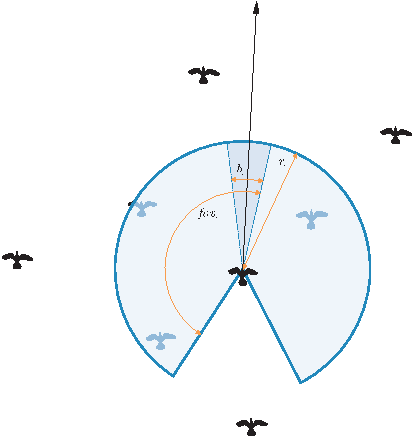
\includegraphics{fig_perception_afd}
	\caption{The perception model used in my fuzzy animat. The black arrow represents the fuzzy digital bird's flight direction. The shaded area represents the visual volume defined by the visual range $r_\textnormal{v}$, per eye visual field $\fov_\textnormal{v}$ and the angle of binocular overlap $b_\textnormal{v}$. The perceived flockmates are depicted in a light blue colour.}
	\label{fig:perception:afd}
\end{figure}
%
At the time being I am using the visual range of seven body lengths and the per eye visual field of \ang{150} with no binocular overlap so that the fuzzy animat has a blind area of \ang{60} behind it, which corresponds closely to the values reported by Heppner \etal\ \cite{heppner:1985}. However, instead of giving full information about the perceived flockmates I give only their \emph{distance}, \emph{angular offset}, relative \emph{difference in flight speed} and relative \emph{difference in flight direction}. I justify this by the fact that using visual perception, a bird can sense only the distance and angular offset of a flockmate, but through cognitive processes and tracking it can judge the relative difference in flight speed (\ie\ if the flockmate is moving faster, slower or with the same speed) and their relative difference in flight direction (\ie\ if the flockmate is flying more to the left, more to the right or in the same direction). Nevertheless in my current implementation the sensed information is still precise (\ie\ exact distance, angular offset, \etc).\footnote{It could be argued that by using this information one can calculate the same precise information as in Reynolds's \cite{reynolds:1999} case, but I strongly object to any mentioning that a bird has precise or full information about its global position in space, absolute flight speed or absolute flight direction.} I reserve the modelling of the binocular overlap and inaccurate visual perception for future work.

Recall that, as in Reynolds's case, in my case the digital universe is homogeneous. Indeed it consists of $n$ fuzzy animats of same kind denoted as $\fautom{B}_1,\ldots,\fautom{B}_n$. Recall that my fuzzy animat's output function is also $\lambda(q)=\langle \vect{p}, \vect{v} \rangle$, where $\vect{p} \in \E$ is the animat's current position in space and $\vect{v} \in \E$ its velocity. This means that at a discrete time step $t \in \set{T}$ the perceivable state of the universe is $u(t)=\langle y_1(t),\ldots,y_n(t) \rangle$, where for all $i=1,\ldots,n$ $y_i=\lambda(q_i(t))$ is the output of fuzzy animat $\fautom{B}_i$ at time step $t$.

As a crisp perception function a fuzzy perception function acts like an interpreter of the perceivable state of the universe and selector of relevant information. But as a contrast to the crisp version it allows modelling inaccurate perception. However, as already said, in the current implementation I model visual perception as accurate.

Let $\fautom{B}_i$ and $\fautom{B}_j$, where $i, j \in \N_n$, be two fuzzy animats from the digital universe and let $q_j=\langle \vect{p}_j, \vect{v}_j, s_j \rangle$ be the current state of fuzzy animat $\fautom{B}_j$ and $y_i=\lambda(q_i)=\langle \vect{p}_i, \vect{v}_i \rangle$ the current output of fuzzy animat $\fautom{B}_i$. Let $\fautom{B}_j$ denote the observed animat. Recall from equation~\eqref{eq:animat:cwr:distance} that the crisp distance of fuzzy animat $\fautom{B}_i$ can be computed as
%
\begin{equation}
	\varepsilon_i=\left\|\vect{p}_i - \vect{p}_j\right\|,
\end{equation}
%
and from equation~\eqref{eq:animat:cwr:angularOffset} that the direction of the offset vector between them (\ie\ their crisp angular offset) can be computed as
%
\begin{equation}
	\varphi_i=\arccos \left( \frac {\vect{v}_j \cdot (\vect{p}_i - \vect{p}_j)}{\left\| \vect{v}_j \right\| \left\| \vect{p}_i - \vect{p}_j \right\|} \right). 
\end{equation}

The crisp difference in flight speed between the observed fuzzy animat $\fautom{B}_j$ and fuzzy animat $\fautom{B}_i$ is on the other hand computed as 
%
\begin{equation}
	\varsigma_i=\left\|\vect{v}_i\right\| - \left\|\vect{v}_j\right\|.
\end{equation}

As already said, the velocity vector $\vect{v}$ gives the relative position changes per coordinate axis in the Cartesian coordinate system. Let $\vect{a}_\textnormal{x}$, $\vect{a}_\textnormal{y}$ and $\vect{a}_\textnormal{z}$ denote the $\mathrm{x}$, $\mathrm{y}$ and $\mathrm{z}$ axis components of vector $\vect{a}$. Then since I am using a two-dimensional Euclidean space $\E=\R^2$, where $\vect{a} \times \vect{b} = \vect{a}_\textnormal{x}\vect{b}_\textnormal{y} - \vect{a}_\textnormal{y}\vect{b}_\textnormal{x}$, the crisp difference in flight direction between the observed fuzzy animat $\fautom{B}_j$ and fuzzy animat $\fautom{B}_i$ is computed as
%
\begin{equation}
	\vartheta_i=\sgn\left(\vect{v}_i \times \vect{v}_j\right)\arccos \left( \frac {\vect{v}_i \cdot \vect{v}_j}{\left\| \vect{v}_i \right\| \left\| \vect{v}_j \right\|} \right),
\end{equation}
%
where $\sgn: \R \mapsto \R$ is the \emph{signum function} defined as 
\begin{equation}
	\sgn x=\left\{
	\begin{array}{rl}
	-1 & \mathrm{iff}\ x < 0\\
	0 & \mathrm{iff}\ x = 0\\
	1 & \mathrm{iff}\ x > 0
	\end{array}
	\right..
\end{equation}

In my model of visual perception the observed animat perceives only the distance, angular offset, difference in flight speed and difference in flight direction of the fuzzy animats that are in its visual volume. This means that the set of visually obtainable information about a fuzzy animat is $\set{I}^\textnormal{v}=\R^4$ and the fuzzy neighbourhood is $\langle\fset{N},\fset{O}\rangle$, where $\fset{N} \in \fpowset{\N_n}$ and $\fset{O} \in \fpowset{\set{I}^\textnormal{v}}^n$. However, since in the current implementation the perception is accurate, the fuzzy set $\fset{N}$ is in fact a crisp set $\set{N} \in \N_n$ and $\fset{O}$ is a crisp value $o \in {(\set{I}^\textnormal{v})}^n$.\footnote{Indeed this can safely be done because fuzzy sets are a generalization of crisp sets and a crisp set $\set{A}$ defined on the universe of discourse $\set{X}$ can always be represented as the fuzzy set $\fset{A}$ whose membership function $\mu_\fset{A}(x)=1\ \mathrm{iff}\ x \in \set{A}$ and $\mu_\fset{A}(x)=0\ \mathrm{iff}\ x \notin \set{A}$, for all $x \in \set{X}$.}

\begin{definition}
	\label{def:fuzzyAnimat:Pv:afd}
	Let $x=\langle y_1,\ldots,y_n\rangle$ be the current perceivable state of the universe, $j$ denote the index of the observed fuzzy animat and let $\set{I}^\textnormal{v}=\R^4$ be the set representing visually obtainable information about a flockmate's distance, angular offset, difference in flight speed and difference in flight direction. Then $\fpowset{\set{P}^\textnormal{v}}=\fpowset{\N_n} \times \fpowset{\set{I}^\textnormal{v}}^n$ and equations~\eqref{eq:fuzzyAnimat:Pv0:afd}--\eqref{eq:fuzzyAnimat:Pv2:afd} define the \emph{fuzzy visual perception function} $\ffunc{P}_\textnormal{v}: \set{X} \times \set{Q} \mapsto \fpowset{\set{P}^\textnormal{v}}$.
	\begin{eqnarray}
		& \ffunc{P}_\textnormal{v}(x,q)=\langle\fset{N},\fset{O}\rangle, & \label{eq:fuzzyAnimat:Pv0:afd} \\
		& \fset{N}=\left\{i|\ i \in \N_n,\ i \neq j,\ \varepsilon_i%(q,y_i)
		 \leq r_\textnormal{v},\ \varphi_i%(q,y_i)
		 < \fov_\textnormal{v} \right\}, & \\ 
		& \fset{O}=\langle \langle \varepsilon_1, \varphi_1, \varsigma_1, \vartheta_1 \rangle, \ldots,
		\langle \varepsilon_n, \varphi_n, \varsigma_n, \vartheta_n \rangle \rangle. & \label{eq:fuzzyAnimat:Pv2:afd}
	\end{eqnarray}
\end{definition}
 
%--
\subsection{Modelling Drives}
Even though, as discussed in subsections~\ref{subsec:birdFlocks:cwr} and \ref{subsec:animat:cwr}, Reynolds in his latest studies \cite{reynolds:1999,reynolds:2000} presented drives\footnote{In his papers he uses the name steering behaviours, but for reasons of consistency and clarity the term drives is used throughout this dissertation.} through the combination of which one can achieve complex behaviours, he states that flocking behaviour can be achieved using only three drives, namely \emph{separation}, \emph{alignment} and \emph{cohesion}. Cohesion simulates attraction toward flockmates and is modelled as the animat's tendency to fly towards the centre of mass of the perceived flockmates. Separation simulates repulsion away from flockmates and is modelled as the animat's tendency to fly away from the perceived flockmates. These two drives (cohesion and separation) represent the attraction-repulsion scheme. Alignment, on the other hand, tries to produce polarization and is modelled as the animat's tendency to change its flight direction and flight speed, so that it corresponds to the average flight direction and flight speed of its perceived flockmates. 

Heppner and Grenander \cite{heppner:1990} (subsections~\ref{subsec:birdFlocks:fhh} and \ref{subsec:animat:fhh}) also modelled three, but different, drives, namely \emph{homing}, \emph{velocity regulation} and \emph{interaction}. Homing simulates the attraction of the roosting point and is modelled as the animat's tendency to fly toward the roosting point. This tendency drops to zero if the animat is close enough (\ie\ a predefined distance) or too far away (\ie\ a predefined distance) from the roosting point. Velocity regulation is modelled as the animat's tendency to fly at a certain predefined preferred speed. Interaction, on the other hand, combines the attraction-repulsion scheme in one single drive and simulates the actual interaction between animats. If two animats are too close (\ie\ a predefined distance) they are repelled, if they are too far (\ie\ a predefined distance) they do not influence each other and if they are anywhere in between, they are attracted.

Attraction towards and repulsion from the flockmates feel natural. After all, their mutual coexistence and importance for the congregation's structure has already been suggested by Okubo \cite{okubo:1980}. Another important feature of groups of uniform density is polarization \cite{parrish:1997a}. Heppner and Grenander \cite{heppner:1990} did not model it specifically, but they mention that in certain cases organized flocks maintaining straight direction of flight emerged. This might be caused by the perception model they used (\ie\ all animats have complete and accurate information about the universe) in conjunction with the velocity regulation drive. Reynolds \cite{reynolds:1987}, however, tries to model polarization through the drive of alignment. 

According to the above discussion I model these three primary drives, the \emph{attraction to flockmates} (fuzzy attraction drive), the \emph{repulsion from flockmates} (fuzzy repulsion drive) and \emph{polarization with flockmates} (fuzzy alignment drive). In the following subsections I will discuss them in greater detail. Note that when modelling attraction to flockmates I do not use a predefined preferred position like the centre of mass \cite{reynolds:1987} and similarly, when modelling polarization with flockmates I do not use a predefined preferred flight speed \cite{heppner:1990}. Instead I let these properties emerge on their own. 

As said before, my fuzzy animat perceives the current state of the universe through visual perception only. At any point in time the fuzzy animat perceives only information about a localized subset of the universe. Since I model the universe as a collection of fuzzy animats, the fuzzy animat thus perceives information about its nearby flockmates. The perceived information includes only distance, angular offset, relative difference in flight direction and relative difference in flight speed of the nearby flockmates. At the time being the perceived information is precise and I reserve modelling inaccurate perception for future work. In addition, I shall suppose that the fuzzy animat can act only by changing its flight speed and/or flight direction.

%-
\subsubsection{The Fuzzy Attraction Drive}
The primary motive of the attraction drive is to stay close to nearby neighbours. Now, imagine a bird that perceives only one neighbour. How would you, in the simplest way possible, describe the action that will keep it close to the perceived neighbour? Assuming that the bird can act only by changing its flight speed and/or flight direction and using common sense most of us would probably state the following:
\begin{enumerate}
	\item in general do not change flight speed or flight direction; \label{dscr:attraction}
	\item when the perceived neighbour is `close enough', change neither flight speed nor flight direction;
	\item when the perceived neighbour is `too far' and `in front', speed up;
	\item when the perceived neighbour is `too far' and anywhere to the `left or behind', turn toward it and slow down;
	\item when the perceived neighbour is `too far' and anywhere to the `right or behind', turn toward it and slow down.
\end{enumerate}

Looking carefully at this description, it can be noticed that the resulting action depends only on the perceived neighbour's distance (\ie\ `close enough', `too far') and position (\ie\ `in front', `left or behind', `right or behind'). But what do `close enough', `too far', `in front', \etc\ mean? Does `in front' perhaps address the precise moment when the perceived neighbour is positioned at an angular offset of \ang{0}? What about \ang{5}, is the perceived neighbour then not `in front'? As it can be seen, `in front' is an imprecise property and constructing a mathematical model from a description that builds on such imprecise properties is a challenging task, which usually requires advanced mathematical skills. Then again, because `close enough', `too far', `in front', \etc\ are imprecise properties and do not represent \emph{crisp values} like \ang{0} or \ang{5}, they can be labelled as vague or \emph{fuzzy values}. Thanks to Zadeh \cite{zadeh:1965}, who introduced \emph{fuzzy sets} (see section~\ref{sec:fuzzyModelling:fuzzySets}), such values can be formally defined.\footnote{In fact, according to the latest fuzzy sets related literature \cite{lee:2004} a fuzzy value is a fuzzy set defined in the real number domain.} Constructing the attraction drive now becomes simple. All that needs to be done is to rewrite the description as a collection of easily understandable \emph{if-then rules} (subsection~\ref{subsec:fuzzyModelling:ifthen}) and the necessary action can be afterwards computed by applying \emph{fuzzy logic} (subsection~\ref{subsec:fuzzyModelling:fuzzyLogic}).

Consider, for example, the fuzzy value `close enough'. As already said, it can be represented with a fuzzy set. In other words, this means that a fuzzy value is uniquely defined by its membership function. In this case, the latter provides the degree to which a real number satisfies the property `close enough' (\ie\ its degree of membership). But because the interpretation of `close enough' is subjective, there is no unique membership function; it is left to the modeller to decide what it should be like. Thus the question is: what did we have in mind with `close enough'? I shall assume that the perceived neighbour is considered as `close enough' if its distance is 40\% of the visual range or less. As the distance increases, the perceived neighbour is considered less and less `close enough' and eventually, when it gets out of the visual range, it is not considered as `close enough' at all. \sidenote{This translates in the membership function that is presented on \fig~\ref{fig:fuzzyAnimat:Da:afd}a.}{v1.1.20050210 [FHH]: these could be explained in more detail for biologists.}
%
\begin{figure}
	\null\vspace*{2mm}\par
	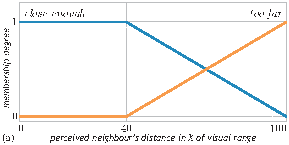
\includegraphics{fig_attraction_a}\hspace*{2mm}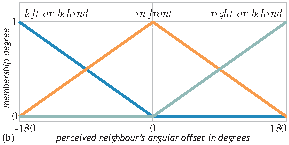
\includegraphics{fig_attraction_b}
	\par\vspace*{2mm}
	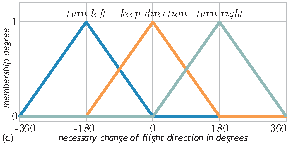
\includegraphics{fig_attraction_c}\hspace*{2mm}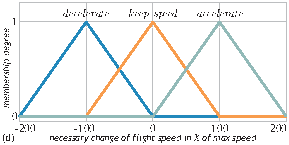
\includegraphics{fig_attraction_d}
	\par\vspace*{2mm}
	\caption{Membership functions of the fuzzy values `close enough', `too far' (a), `in front', `left or behind', `right or behind' (b), `turn left', `keep direction', `turn right' (c), `decelerate', `keep speed', `accelerate' (d) for the case of the attraction drive.}
	\label{fig:fuzzyAnimat:Da:afd}
\end{figure}
%
However, this is only one of the many possible interpretations of `close enough' and an interesting question is: when does a bird consider its neighbour to be `close enough'? Here comes into play the expertise of field ornithologists, who could use a tool such as this to translate their observational knowledge into simulation models.

In a similar fashion the fuzzy values `too far', `in front', `left or behind' and `right or behind' can be defined (\figs~\ref{fig:fuzzyAnimat:Da:afd}a and b). Furthermore, by introducing the fuzzy values `keep direction', `turn left', `turn right', `keep speed', `accelerate' and `decelerate' (\figs~\ref{fig:fuzzyAnimat:Da:afd}c and d) to represent the actions of keeping the same flight direction, performing a left turn and performing a right turn, keeping the same flight speed, accelerating and decelerating, the initial description can be rewritten in the form of a set of if-then rules denoted as the \emph{attraction fuzzy rule base}.

{\footnotesize
\begin{tabbing}
	\quad \= \frule{a1}: \quad \= \kwd{if} \=(\fvar{distance} \kwd{is} \fval{close enough}) \kwd{then} (\fvar{flight direction} \kwd{is} \fval{keep direction}), \\
	\> \frule{a2}: \> \kwd{if} (\fvar{distance} \kwd{is} \fval{too far}) \kwd{then} (\fvar{flight direction} \kwd{is} \fval{keep direction}), \\
	\> \frule{a3}: \> \kwd{if} (\fvar{distance} \kwd{is} \fval{close enough}) \kwd{then} (\fvar{flight speed} \kwd{is} \fval{keep speed}), \\
	\> \frule{a4}: \> \kwd{if} (\fvar{distance} \kwd{is} \fval{too far}) \kwd{then} (\fvar{flight speed} \kwd{is} \fval{keep speed}), \\
	\> \frule{a5}: \> \kwd{if} (\fvar{distance} \kwd{is} \fval{too far}) \kwd{and} (\fvar{position} \kwd{is} \fval{in front}) \kwd{then} (\fvar{flight speed} \kwd{is} \fval{accelerate}), \\
	\> \frule{a6}: \> \kwd{if} (\fvar{distance} \kwd{is} \fval{too far}) \kwd{and} (\fvar{position} \kwd{is} \fval{left or behind}) \kwd{then} (\fvar{flight direction} \kwd{is} \fval{turn left}), \\
	\> \frule{a7}: \> \kwd{if} (\fvar{distance} \kwd{is} \fval{too far}) \kwd{and} (\fvar{position} \kwd{is} \fvar{left or behind}) \kwd{then} (\fvar{flight speed} \kwd{is} \fval{decelerate}), \\
	\> \frule{a8}: \> \kwd{if} (\fvar{distance} \kwd{is} \fval{too far}) \kwd{and} (\fvar{position} \kwd{is} \fvar{right or behind}) \kwd{then} (\fvar{flight direction} \kwd{is} \fval{turn right}), \\
	\> \frule{a9}: \> \kwd{if} (\fvar{distance} \kwd{is} \fval{too far}) \kwd{and} (\fvar{position} \kwd{is} \fvar{right or behind}) \kwd{then} (\fvar{flight speed} \kwd{is} \fval{decelerate}).
\end{tabbing}
}

The first four rules from the attraction fuzzy rule base (\ie\ rules \frule{a1}--\frule{a4}) model the assumption that a bird in general tends not to change its flight direction or flight speed; item (1) in the description on page~\pageref{dscr:attraction}. Rules \frule{a2} and \frule{a4} model the assumption that a bird, in order to keep close to a neighbour that is already close enough, does not need to do anything; item (2). Rule \frule{a5} models the assumption that a bird, in order to catch up with a neighbour that is in front of it but too far, needs only to speed up; item (3). Finally, the last four rules (\frule{a6}--\frule{a9}) model the assumption that a bird, in order to get close to a neighbour that is too far but positioned sideways or behind, needs to turn toward it and slow down; items (4) and (5). 

The attraction fuzzy rule base can be used to model the fuzzy animat's attraction drive. When the fuzzy animat perceives only one neighbour, its uncertain action (\ie\ the changes in flight direction and/or flight speed as fuzzy sets) is computed by applying fuzzy logic on each of the rules and combining the rule outputs. The resulting action will keep the animat close to the perceived neighbour. When the fuzzy animat perceives more than one neighbour the rules are evaluated for each neighbour independently (\ie\ as if the animat perceived only that neighbour) and all outputs are combined (see section~\ref{sec:fuzzyAnimat:decision}). The resulting action is a combination that will satisfy the fuzzy animat's drive to keep close to all of the perceived neighbours. In any case the resulting uncertain action is given through the fuzzy set representing the required uncertain change in flight direction and the fuzzy set representing the required uncertain change in flight speed.

Recall that my fuzzy animat uses only one fuzzy perception function (\ie\ the fuzzy visual perception function---definition~\ref{def:fuzzyAnimat:Pv:afd}). This means that the set representing uncertain information that can be obtained from the current perceivable state of the universe is $\fpowset{\set{P}}=\fpowset{\set{P}^\textnormal{v}}=\fpowset{\N_n} \times \fpowset{\set{I}^\textnormal{v}}^n$ and that $\set{I}^\textnormal{v}=\R^4$. Furthermore, recall that the perception is accurate, which means that the fuzzy neighbourhood $\langle \fset{N}, \fset{O} \rangle \in \fpowset{\set{P}}$ is crisp (\ie\ the fuzzy sets $\fset{N} \in \fpowset{\N_n}$ and $\fset{O} \in \fpowset{\set{I}^\textnormal{v}}^n$ represent crisp sets). This means that the uncertain information about fuzzy animat $\fautom{B}_i$ is actually represented by the quadruple $\langle \varepsilon_i, \varphi_i, \varsigma_i, \vartheta_i \rangle \in \fpowset{\set{I}^\textnormal{v}}$ (\ie\ the crisp distance, crisp angular offset, crisp difference in flight speed and crisp difference in flight direction between the observed fuzzy animat and fuzzy animat $\fautom{B}_i$). In addition it also means that the fuzzy set of indexes of the relevant fuzzy animats is a crisp set (\ie\ $\mu_\fset{N}(i) \in \left\{0,1\right\}$ for all $i \in \N_n$). 

As discussed earlier, my fuzzy animat can act only by changing its flight direction and/or flight speed. In other words: the set representing all possible actions is $\set{A}=\R^2$. The uncertain action (\ie\ the required uncertain flight direction change given as the fuzzy set $\fset{D} \in \fpowset{\R}$ and the required uncertain flight speed change given as the fuzzy set $\fset{S} \in \fpowset{\R}$) that with respect to the perceived uncertain information about the state of the universe $\langle \fset{N}, \fset{O} \rangle \in \fpowset{\set{P}}$ and the current state of the fuzzy animat $q$ satisfy the attraction drive is therefore given as $\fset{A}_\textnormal{a}=\langle \fset{D}_\textnormal{a}, \fset{S}_\textnormal{a} \rangle \in \fpowset{\set{A}}$.

\begin{definition}
	\label{def:fuzzyAnimat:Da:afd} 
	Let the fuzzy neighbourhood returned by the visual perception function be $\fset{P}_\textnormal{v}=\langle \fset{N}, \fset{O} \rangle \in \fpowset{\set{P}}$, where $\fset{N}$ is the fuzzy set of indexes of the relevant fuzzy animats and $\fset{O} \in \fpowset{\set{I}^\textnormal{v}}^n$ represents uncertain information about the existing fuzzy animats. The \emph{fuzzy attraction drive function} $\ffunc{D}_\textnormal{a}: \fpowset{\set{P}} \times \set{Q} \mapsto \fpowset{\set{A}}$ can therefore be written as
	\begin{equation}
		\ffunc{D}_\textnormal{a}(\fset{P}_\textnormal{v},q)=%\langle \fset{D}_\textnormal{a}, \fset{S}_\textnormal{a} \rangle =
		 \biguplus_{\forall i(\mu_\fset{N}(i)=1)} \mathcal{L}_\texttt{a}(\langle \varepsilon_i, \varphi_i, \varsigma_i, \vartheta_i \rangle),
	\end{equation}
	where $\mathcal{L}_\texttt{a}: \fpowset{\set{I}^\textnormal{v}} \mapsto \fpowset{\set{A}}$ denotes the application of fuzzy logic on the attraction fuzzy rule base with $\fvar{distance}=\varepsilon_i$ and $\fvar{position}=\varphi_i$.
\end{definition}

%-
\subsubsection{The Fuzzy Repulsion Drive}
The primary motive of the repulsion drive is to stay away from collisions. I shall again assume that the hypothetical bird perceives only one neighbour, except that this time I am interested in the action that will keep it away from colliding with that neighbour. Using common sense, most of us would describe the bird's behaviour in the following way:
\begin{enumerate}
	\item in general do not change flight speed or flight direction;
	\item when the perceived neighbour is `far enough', change neither flight speed nor flight direction;
	\item when the perceived neighbour is `too close' and anywhere `behind', speed up;
	\item when the perceived neighbour is `too close' and `in front or right', turn away from it and slow down;
	\item when the perceived neighbour is `too close' and `in front or left', turn away from it and slow down.
\end{enumerate}

Once more it can be noticed that in the description the resulting action depends only on the perceived neighbour's distance and position. Therefore, as in the case of the attraction drive, I shall first define the fuzzy values `far enough', `too close', `behind', `in front or right' and `in front or left' (\figs~\ref{fig:fuzzyAnimat:Dr:afd}a and b). 
%
\begin{figure}
	\null\vspace*{2mm}\par
	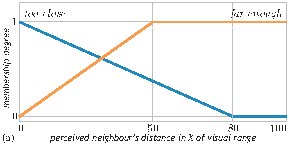
\includegraphics{fig_repulsion_a}\hspace*{2mm}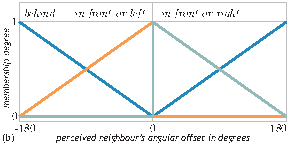
\includegraphics{fig_repulsion_b}
	\par\vspace*{2mm}
	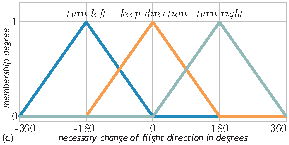
\includegraphics{fig_repulsion_c}\hspace*{2mm}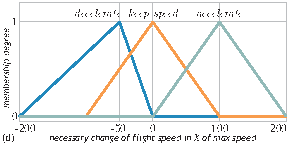
\includegraphics{fig_repulsion_d}
	\par\vspace*{2mm}
	\caption{Membership functions of the fuzzy values `too close', `far enough' (a), `behind', `in front or left', `in front or right' (b), `turn left', `keep direction', `turn right' (c), `decelerate', `keep speed', `accelerate' (d) for the case of the repulsion drive.}
	\label{fig:fuzzyAnimat:Dr:afd}
\end{figure}
%
Then, assuming that the bird can act only by changing its flight direction and/or flight speed, I shall introduce the fuzzy values that represent the actions of keeping the same flight direction, performing a left turn, \etc\ (\figs~\ref{fig:fuzzyAnimat:Dr:afd}c and d). After completing these two steps the initial description can be rewritten in the form of a set of if-then rules that I shall denote as the \emph{repulsion fuzzy rule base}.

{\footnotesize
\begin{tabbing}
	\quad \= \frule{r1}: \quad \= \kwd{if} \=(\fvar{distance} \kwd{is} \fval{far enough}) \kwd{then} (\fvar{flight direction} \kwd{is} \fval{keep direction}), \\
	\> \frule{r2}: \> \kwd{if} (\fvar{distance} \kwd{is} \fval{too close}) \kwd{then} (\fvar{flight direction} \kwd{is} \fval{keep direction}), \\
	\> \frule{r3}: \> \kwd{if} (\fvar{distance} \kwd{is} \fval{far enough}) \kwd{then} (\fvar{flight speed} \kwd{is} \fval{keep speed}), \\
	\> \frule{r4}: \> \kwd{if} (\fvar{distance} \kwd{is} \fval{too close}) \kwd{then} (\fvar{flight speed} \kwd{is} \fval{keep speed}), \\
	\> \frule{r5}: \> \kwd{if} (\fvar{distance} \kwd{is} \fval{too close}) \kwd{and} (\fvar{position} \kwd{is} \fval{behind}) \kwd{then} (\fvar{flight speed} \kwd{is} \fval{accelerate}), \\
	\> \frule{r6}: \> \kwd{if} (\fvar{distance} \kwd{is} \fval{too close}) \kwd{and} (\fvar{position} \kwd{is} \fval{in front or left}) \kwd{then} (\fvar{flight direction} \kwd{is} \fval{turn right}), \\
	\> \frule{r7}: \> \kwd{if} (\fvar{distance} \kwd{is} \fval{too close}) \kwd{and} (\fvar{position} \kwd{is} \fvar{in front or left}) \kwd{then} (\fvar{flight speed} \kwd{is} \fval{decelerate}), \\
	\> \frule{r8}: \> \kwd{if} (\fvar{distance} \kwd{is} \fval{too close}) \kwd{and} (\fvar{position} \kwd{is} \fvar{in front or right}) \kwd{then} (\fvar{flight direction} \kwd{is} \fval{turn left}), \\
	\> \frule{r9}: \> \kwd{if} (\fvar{distance} \kwd{is} \fval{too close}) \kwd{and} (\fvar{position} \kwd{is} \fvar{in front or right}) \kwd{then} (\fvar{flight speed} \kwd{is} \fval{decelerate}).
\end{tabbing}
}

As in the case of the attraction drive, the repulsion fuzzy rule base can be used to model the fuzzy animat's repulsion drive. In other words, for each of the perceived neighbours the fuzzy animat applies fuzzy logic on each of the rules from the repulsion fuzzy rule base and works out the uncertain action that should be taken to keep away from colliding with any of the perceived neighbours (see section~\ref{sec:fuzzyAnimat:decision}).

\begin{definition}
	\label{def:fuzzyAnimat:Dr:afd} 
	Let the fuzzy neighbourhood returned by the visual perception function be $\fset{P}_\textnormal{v}=\langle \fset{N}, \fset{O} \rangle \in \fpowset{\set{P}}$, where $\fset{N}$ is the fuzzy set of indexes of the relevant fuzzy animats and $\fset{O} \in \fpowset{\set{I}^\textnormal{v}}^n$ represents uncertain information about the existing fuzzy animats. The \emph{fuzzy repulsion drive function} $\ffunc{D}_\textnormal{r}:\fpowset{\set{P}} \times \set{Q} \mapsto \fpowset{\set{A}}$ can therefore be written as
	\begin{equation}
	\ffunc{D}_\textnormal{r}(\fset{P}_\textnormal{v},q)=%\langle \fset{D}_\textnormal{r}, \fset{S}_\textnormal{r} \rangle =
	 \biguplus_{\forall i(\mu_\fset{N}(i)=1)} \mathcal{L}_\texttt{r}(\langle \varepsilon_i, \varphi_i, \varsigma_i, \vartheta_i \rangle),
	\end{equation}
	where $\mathcal{L}_\texttt{r}: \fpowset{\set{I}^\textnormal{v}} \mapsto \fpowset{\set{A}}$ denotes the application of fuzzy logic on the repulsion fuzzy rule base with $\fvar{distance}=\varepsilon_i$ and $\fvar{position}=\varphi_i$.
\end{definition}

%-
\subsubsection{The Fuzzy Alignment Drive}
The alignment drive's motive is to achieve polarization with flockmates (\ie\ to keep approximately the same flight speed and flight direction as the perceived flockmates). If it is yet again assumed that the hypothetical bird perceives only one neighbour then the necessary actions can be described as follows:

\begin{enumerate}
	\item in general do not change flight speed or flight direction;
	\item when the perceived neighbour is `too far' or `too close', change neither flight speed nor flight direction;
	\item when the perceived neighbour is at a `good' distance and flying in the `same direction', keep flight direction;
	\item when the perceived neighbour is at a `good' distance but flying more to the `left', turn left;
	\item when the perceived neighbour is at a `good' distance but flying more to the `right', turn right;
	\item when the perceived neighbour is at a `good' distance and flying with the `same speed', keep flight speed;
	\item when the perceived neighbour is at a `good' distance but flying `slower', slow down;
	\item when the perceived neighbour is at a `good' distance but flying `faster', speed up.
\end{enumerate}

\begin{figure}
	\null\vspace*{2mm}\par
	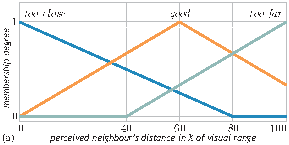
\includegraphics{fig_alignment_a}\hspace*{2mm}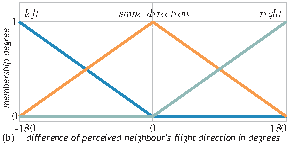
\includegraphics{fig_alignment_b}
	\par\vspace*{2mm}
	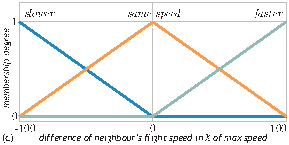
\includegraphics{fig_alignment_c}
	\par\vspace*{2mm}
	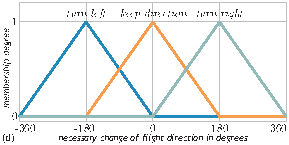
\includegraphics{fig_alignment_d}\hspace*{2mm}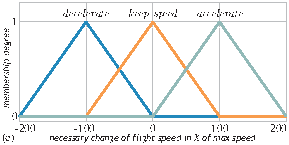
\includegraphics{fig_alignment_e}
	\par\vspace*{2mm}
	\caption{Membership functions of the fuzzy values `too close', `good', `too far' (a), `left', `same direction', `right' (b), `slower', `same speed', `faster' (c), `turn left', `keep direction', `turn right' (d), `decelerate', `keep speed', `accelerate' (e) for the case of the alignment drive.}
	\label{fig:fuzzyAnimat:Dp:afd}
\end{figure}

As a contrast to the attraction and repulsion drives it can be noticed that in this case the action depends on the perceived neighbour's distance, difference in flight direction and difference in flight speed. After the definition and introduction of the required fuzzy values (\fig~\ref{fig:fuzzyAnimat:Dp:afd}) the initial description can be rewritten in the form of the \emph{alignment fuzzy rule base}.

{\footnotesize
\begin{tabbing}
	\quad \= \frule{p1}: \quad \= \kwd{if} \=(\fvar{distance} \kwd{is} \fval{too far}) \kwd{then} (\fvar{flight direction} \kwd{is} \fval{keep direction}), \\
	\> \frule{p2}: \> \kwd{if} (\fvar{distance} \kwd{is} \fval{too close}) \kwd{then} (\fvar{flight direction} \kwd{is} \fval{keep direction}), \\
	\> \frule{p3}: \> \kwd{if} (\fvar{distance} \kwd{is} \fval{too far}) \kwd{then} (\fvar{flight speed} \kwd{is} \fval{keep speed}), \\
	\> \frule{p4}: \> \kwd{if} (\fvar{distance} \kwd{is} \fval{too close}) \kwd{then} (\fvar{flight speed} \kwd{is} \fval{keep speed}), \\
	\> \frule{p5}: \> \kwd{if} (\fvar{distance} \kwd{is} \fval{good}) \kwd{and} (\fvar{direction} \kwd{is} \fval{same direction}) \kwd{then} (\fvar{flight direction} \kwd{is} \fval{keep direction}), \\
	\> \frule{p6}: \> \kwd{if} (\fvar{distance} \kwd{is} \fval{good}) \kwd{and} (\fvar{direction} \kwd{is} \fval{left}) \kwd{then} (\fvar{flight direction} \kwd{is} \fval{turn left}), \\
	\> \frule{p7}: \> \kwd{if} (\fvar{distance} \kwd{is} \fval{good}) \kwd{and} (\fvar{direction} \kwd{is} \fval{right}) \kwd{then} (\fvar{flight direction} \kwd{is} \fval{turn right}), \\
	\> \frule{p8}: \> \kwd{if} (\fvar{distance} \kwd{is} \fval{good}) \kwd{and} (\fvar{speed} \kwd{is} \fval{same speed}) \kwd{then} (\fvar{flight speed} \kwd{is} \fval{keep speed}), \\
	\> \frule{p9}: \> \kwd{if} (\fvar{distance} \kwd{is} \fval{good}) \kwd{and} (\fvar{speed} \kwd{is} \fvar{slower}) \kwd{then} (\fvar{flight speed} \kwd{is} \fval{decelerate}), \\
	\> \frule{p10}: \> \kwd{if} (\fvar{distance} \kwd{is} \fval{good}) \kwd{and} (\fvar{speed} \kwd{is} \fvar{faster}) \kwd{then} (\fvar{flight speed} \kwd{is} \fval{accelerate}).
\end{tabbing}
}
 
Yet again the alignment fuzzy rule base can be used to model the fuzzy animat's alignment drive. That is, by applying fuzzy logic on it, the fuzzy animat can work out the uncertain action that should be taken in order to keep approximately the same flight speed and flight direction as the perceived neighbours (see section~\ref{sec:fuzzyAnimat:decision}).

\begin{definition}
	\label{def:fuzzyAnimat:Dp:afd} 
	Let the fuzzy neighbourhood returned by the visual perception function be $\fset{P}_\textnormal{v}=\langle \fset{N}, \fset{O} \rangle \in \fpowset{\set{P}}$, where $\fset{N}$ is the fuzzy set of indexes of the relevant fuzzy animats and $\fset{O} \in \fpowset{\set{I}^\textnormal{v}}^n$ represents uncertain information about the existing fuzzy animats. The \emph{fuzzy alignment drive function} $\ffunc{D}_\textnormal{p}: \fpowset{\set{P}} \times \fset{Q} \mapsto \fpowset{\set{A}}$ can therefore be written as
	\begin{equation}
		\ffunc{D}_\textnormal{p}(\fset{P}_\textnormal{v},q)=%\langle \fset{D}_\textnormal{p}, \fset{S}_\textnormal{p} \rangle =
		 \biguplus_{\forall i(\mu_\fset{N}(i)=1)} \mathcal{L}_\texttt{p}(\langle \varepsilon_i, \varphi_i, \varsigma_i, \vartheta_i \rangle),
	\end{equation}
	where $\mathcal{L}_\texttt{p}: \fpowset{\set{I}^\textnormal{v}} \mapsto \fpowset{\set{A}}$ denotes the application of fuzzy logic on the alignment fuzzy rule base, where $\fvar{distance}=\varepsilon_i$, $\fvar{speed}=\varsigma_i$ and $\fvar{direction}=\vartheta_i$.
\end{definition}

%--
\subsection{Modelling Action Selection}
As already discussed, the action selection process simulates the animal's neurological process of selecting the sequence of muscular movements that will accomplish the actions that result from its drives. This process combines, prioritizes, and arbitrates between potentially conflicting actions. Similar to Reynolds \cite{reynolds:1987,reynolds:1999} (subsection~\ref{subsec:animat:cwr}) and Heppner and Grenander \cite{heppner:1990} (subsection~\ref{subsec:animat:fhh}), in my study I do not model the musculoskeletal structure of a real bird and model the action selection mechanism as a simple combination of the actions that result from the animat's drives. In other words, for each of the animat's drives a vector is calculated that represents the force needed to accomplish the required action. These forces are then combined by using a weighted sum and the resulting vector used to calculate the animat's new flight speed and flight direction. This calculation is subjected to a set of constraints modelling conservation of momentum, viscous damping and the animal's finite amount of available energy. The same approach named geometrical flight was already used by Reynolds \cite{reynolds:1987,reynolds:1999} (see subsection~\ref{subsec:animat:cwr}). Heppner and Grenander \cite{heppner:1990}, who represented actions as vectors (see subsection~\ref{subsec:animat:fhh}), used a similar approach and modelled action selection as a simple weighted sum. However, apart from the Poisson stochastic process modelling the effects of wind gusts and random local disturbances, they did not apply any additional constraints. 

To sum up, my fuzzy animat is based on a point mass approximation. The same approach, named a point mass vehicle model, was used by Reynolds \cite{reynolds:1987,reynolds:1999} (see subsection~\ref{subsec:animat:cwr}). This means that my fuzzy animat's physics is also based on forward Euler integration \cite{parent:2002,reynolds:1999}. As said, for each of the fuzzy animat's three fuzzy drives (\ie\ the fuzzy attraction, fuzzy repulsion and fuzzy alignment drive) a vector is calculated that represents the force needed to accomplish the required action. However, in my case, the uncertain action resulting from a fuzzy drive gives the required uncertain change in flight direction and the required uncertain change in flight speed as fuzzy sets. This means that each of the two fuzzy sets needs first to be converted into a single (crisp) value which, in some sense, is the best representative of the fuzzy set. This is achieved through defuzzification (see subsection~\ref{subsec:fuzzyModelling:fuzzyRuleBase}). The defuzzified values are then used to compute the forces required to initiate the desired changes and these are afterwards combined by using a weighted sum. \sidenote{The weights have been chosen so as to give the highest priority to the fuzzy repulsion drive, followed by the fuzzy alignment drive, and the lowest priority to the fuzzy attraction drive.}{v1.0.20050124 [MM]: provide an explanation why so.\\v1.3.20050407 [BZ]: Why? Any analysis on what would changes cause?\\v1.4.20050412 [ILB]: This was based both on the weights employed by Reynolds and on the analysis of the importance of the separation, alignment and cohesion drive used in his model \cite{lebar_bajec:2002,lebar_bajec:2003a}.} The resulting vector is used to calculate the fuzzy animat's new flight speed and flight direction. In other words, the resulting force (limited by the fuzzy animat's available force) is applied to the fuzzy animat's point mass. This produces an acceleration equal to the force divided by the fuzzy animat's mass. The acceleration is then added to the fuzzy animat's current velocity vector and truncated by the maximum achievable speed. Finally the fuzzy animat's new position is computed by adding the new velocity vector to the fuzzy animat's current position. 

Let $\vect{a} \in \E$ be a vector. Then since I am using the two-dimensional Euclidean vector space $\E=\R^2$ the rotation of vector $\vect{a}$ for the angle $\alpha$ is defined as
%
\begin{equation}
	R(\vect{a}, \alpha) = \left(\vect{a}_\textnormal{x}\cos\alpha + \vect{a}_\textnormal{y}\sin\alpha\right)\vect{e}_\textnormal{i} + \left(-\vect{a}_\textnormal{x}\sin\alpha + \vect{a}_\textnormal{y}\cos\alpha\right)\vect{e}_\textnormal{j},
\end{equation}
%
where $\vect{e}_\textnormal{i}$, $\vect{e}_\textnormal{j}$ are the $\mathrm{x}$ and $\mathrm{y}$ axis unit vectors of the Cartesian coordinate system.

Furthermore, if $a \in \R^+$ is used to represent the maximal size of vector $\vect{a}$, equation~\eqref{eq:truncation} still holds, and truncation of vector $\vect{a}$ so that its size is lower or equal $a$ is computed as
%
\begin{equation}
	\lfloor\vect{a}\rceil^{a} = \min(\left\|\vect{a}\right\|, a) \vect{a}^0. \nonumber
\end{equation}

Let $\fset{A}=\langle \fset{D}, \fset{S} \rangle \in \fpowset{\set{A}}$ represent the desired uncertain action returned by one of the fuzzy drive functions from definitions~\ref{def:fuzzyAnimat:Da:afd}--\ref{def:fuzzyAnimat:Dp:afd}. Let the fuzzy set $\fset{D}$ represent the desired uncertain flight direction change and let the fuzzy set $\fset{S}$ the desired uncertain flight speed change. Let the current state of the observed fuzzy animat be $q=\langle \vect{p}, \vect{v}, s \rangle$, where $\vect{p}$ is the fuzzy animat's current position in space, $\vect{v}$ its velocity and $s$ the modelled animal's internal state defined by definition~\ref{def:fuzzyAnimat:s:afd}. Then the mapping $F: \fpowset{\set{A}} \times \set{Q} \mapsto \E$ given by equation~\eqref{eq:fuzzyAnimat:Sws:force:afd} computes the force required to initiate the desired change in flight speed and/or flight direction.
\begin{equation}
	F(\fset{A},q)=\left\lfloor\max(\left\|\vect{v}\right\|+\cog\fset{S},0)R(\vect{v}^0,\cog\fset{D})\right\rceil^{v_\textnormal{M}}-\vect{v}. \label{eq:fuzzyAnimat:Sws:force:afd}
\end{equation}

\begin{definition}
	\label{def:fuzzyAnimat:Sws:afd}
	Let the current state of the fuzzy animat be $q=\langle\vect{p},\vect{v},s\rangle$, where the modelled animal's internal state $s$ is defined by definition~\ref{def:fuzzyAnimat:s:afd}. Let the computed desired uncertain actions be $\langle \fset{A}_\textnormal{a},\fset{A}_\textnormal{r},\fset{A}_\textnormal{p}\rangle$. Let $w_\textnormal{a}$, $w_\textnormal{r}$ and $w_\textnormal{p}$ represent the weight of the fuzzy attraction, fuzzy repulsion and fuzzy alignment drive respectively and let $dt$ represent the simulation step. Then the \emph{fuzzy weighted sum action selection function} $\ffunc{S}_\textnormal{ws}: \fpowset{\set{A}} \times \set{Q} \mapsto \set{Q}$ is defined as
	\begin{equation}
		S_\textnormal{ws}(\langle \fset{A}_\textnormal{a},\fset{A}_\textnormal{r},\fset{A}_\textnormal{p}\rangle, q) = \langle\vect{p}', \vect{v}', s\rangle, \label{eq:fuzzyAnimat:Sws0:afd}
	\end{equation}
	\begin{equation}
		\vect{v}' = \left\lfloor {\vect{v} + \frac{\left\lfloor w_\textnormal{a}F(\fset{A}_\textnormal{a},q) + w_\textnormal{r}F(\fset{A}_\textnormal{r},q) + w_\textnormal{p}F(\fset{A}_\textnormal{p},q) \right\rceil^{f_\textnormal{M}}}{m}}dt \right\rceil^{v_\textnormal{M}},
	\end{equation}
	\begin{equation}
		\vect{p}' = \vect{p} + \vect{v}'dt. \label{eq:fuzzyAnimat:Sws2:afd}
	\end{equation}
\end{definition}
 
%--
\subsection{A Wingbeat of the Fuzzy Digital Bird}
\label{sec:fuzzyAnimat:decision}
In the previous sections a formal definition of a fuzzy digital bird was presented. With a collection of the latter, a fuzzy model for a computer simulation of bird flocking can be constructed. This section provides an example of the steps taken in processing a single decision. The main emphasis is given to the computation of the fuzzy drives.

Let the current state of the digital universe be such that the observed fuzzy animat perceives only two neighbours. Let neighbour $\fautom{B}_1$ be 80\% of the observed fuzzy animat's visual range away with an angular offset of \ang{-30} and neighbour $\fautom{B}_2$ 60\% of the visual range away with an angular offset of \ang{-110} (\fig~\ref{fig:attraction:FLS:ini}). For reasons of simplicity I shall assume that they are all flying in the same direction and with the same flight speed. 

\begin{figure}
	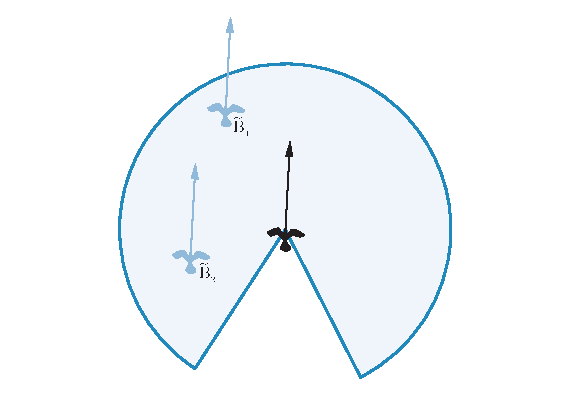
\includegraphics{fig_attractionFLSini}
	\caption{The observed fuzzy animat perceives two neighbours, one of which is 80\% of the visual range away with an angular offset of \ang{-30} ($\fautom{B}_1$), and the other is 60\% of the visual range away with an angular offset of \ang{-110} ($\fautom{B}_2$). All fuzzy animats have the same flight direction and flight speed (black and blue arrows).}
	\label{fig:attraction:FLS:ini}
\end{figure}

By computing the fuzzy attraction, fuzzy repulsion and fuzzy alignment drive (\ie\ applying fuzzy logic on the attraction, repulsion and alignment fuzzy rule bases) the observed fuzzy animat computes three independent actions (\ie\ uncertain flight direction and/or flight speed changes). These actions together will satisfy its drives to stay close to the perceived neighbours, keep away from colliding with them and fly in approximately the same direction and flight speed. With the fuzzy weighted sum action selection function the fuzzy animat then combines, prioritizes and arbitrates these actions and computes the flight direction and/or flight speed change to be taken in the following time step. 

Even though all fuzzy drives can be computed simultaneously, let me start with the fuzzy attraction drive. For each of the perceived neighbours the fuzzy rule base is evaluated independently (\ie\ as if the fuzzy animat perceived only one neighbour) and all outputs are later combined. Now, recall that the action that satisfies the fuzzy attraction drive depends only on the perceived neighbour's distance and position. Because all of the perceived information is precise, for neighbour $\fautom{B}_1$, \fvar{distance} is the crisp value 80\% of the visual range and \fvar{position} is the crisp value \ang{-30}. 

First let me compute the necessary change in flight direction (\ie\ evaluate rules \frule{a1}, \frule{a2}, \frule{a6} and \frule{a8} from the attraction fuzzy rule base). It is easy to notice that rules \frule{a1} and \frule{a2} have the same consequent (\ie\ `\fvar{distance} \kwd{is} \fval{keep direction}'). Because of this their antecedents can be joined, using the logical operator `\kwd{or}', and interpreted as a single rule. To assess the degree of truth of the compound antecedent the degrees of truth of the individual antecedents must first be computed and then the fuzzy logic operator `\kwd{or}' must be applied. 

Let $\statement{A}_1$ denote the antecedent of rule \frule{a1} (\ie\ `\fvar{distance} \kwd{is} \fval{close enough}') and $\statement{A}_2$ the antecedent of rule \frule{a2} (\ie\ `\fvar{distance} \kwd{is} \fval{too far}'). Recall that as distance is a crisp value, the degrees of truth of $\statement{A}_1$ and $\statement{A}_2$ are given by the degree of membership of distance in the corresponding fuzzy sets (see subsection~\ref{subsec:fuzzyModelling:fuzzyLogic}). Therefore, if $d$ is used to denote the value of distance, $\fset{C}$ to denote the fuzzy set `close enough' and $\fset{F}$ the fuzzy set `too far', then
%
\begin{equation}
	\begin{array}{ll}
	T(\statement{A}_1)=\mu_\fset{C}(d)=\mu_\fset{C}(80)=0.33, \\
	T(\statement{A}_2)=\mu_\fset{F}(d)=\mu_\fset{F}(80)=0.67.
	\end{array}
\end{equation}
%
Since in this dissertation the logical operator `\kwd{or}' is interpreted as maximum fuzzy union, the degree of truth of the compound antecedent is 
%
\begin{equation}
	T(\statement{A}_1\ \kwd{or}\ \statement{A}_2)=\max(T(\statement{A}_1),T(\statement{A}_2))=\max(0.33,0.67)=0.67.
\end{equation}
%
Recall that the degree of truth of the antecedent implies the degree of truth of the conclusion, and that fuzzy implication modifies the output fuzzy set (see subsection~\ref{subsec:fuzzyModelling:ifthen}). Let $\mu_\fset{K}$ denote the fuzzy set `keep direction'. Then, as this dissertation makes use of product fuzzy implication, which modifies the output fuzzy set by squashing it, the membership function of the modified output fuzzy set that results from rules \frule{a1} and \frule{a2} is given by
%
\begin{equation}
	\mu_{\fset{K}'}(r)=T(\statement{A}_1\ \kwd{or}\ \statement{A}_2) \cdot \mu_\fset{K}(r)=0.67 \cdot \mu_\fset{K}(r).
\end{equation}

\begin{figure}
	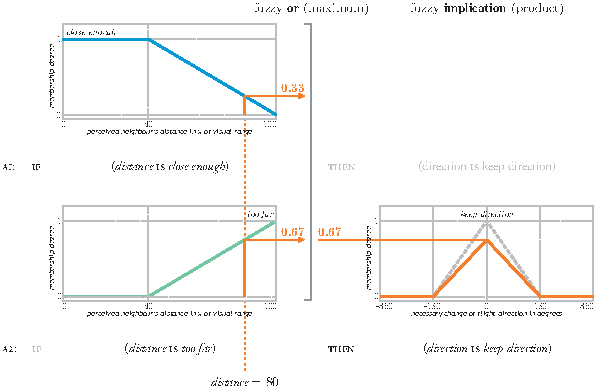
\includegraphics{fig_attractionFLSa1+a2}
	\caption{Graphical representation of the evaluation of rules \frule{a1} and \frule{a2} for the case when the perceived neighbour is 80\% of the visual range away with an angular offset of \ang{-30}. The left half shows the evaluation of the degrees of truth of the antecedents and the right part the modification of the output fuzzy set.}
	\label{fig:attraction:FLS:a1+a2}
\end{figure}

A graphical representation of the above described evaluation process is presented in figure~\ref{fig:attraction:FLS:a1+a2}. The left half shows the evaluation of the antecedents' degrees of truth, while the right shows the modification of the output fuzzy set.

Rules \frule{a6} and \frule{a8} have different consequents, which means that they, even though they can be evaluated simultaneously, cannot be treated as a single rule. It can be noticed, however, that their antecedents have multiple parts. In both cases the antecedent is composed of two conditions joined by the logical operator `\kwd{and}'. This means that to evaluate the degree of truth of the antecedent the degrees of truth of the individual conditions must first be computed and then the fuzzy logic operator `\kwd{and}' must be applied. A graphical representation of the evaluation process is presented in figure~\ref{fig:attraction:FLS:a6+a8}.

\begin{figure}
	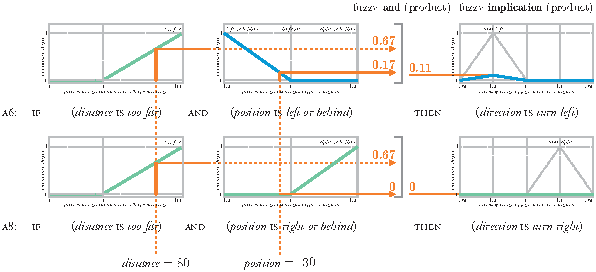
\includegraphics{fig_attractionFLSa6+a8}
	\caption{Graphical representation of the evaluation of rules \frule{a6} and \frule{a8} for the case when the perceived neighbour is 80\% of the visual range away with an angular offset of \ang{-30}. The left half shows the evaluation of the degrees of truth of the antecedents and the right part the modification of the output fuzzy sets.}
	\label{fig:attraction:FLS:a6+a8}
\end{figure}

For rule \frule{a6} let $\statement{A}_{61}$ denote condition `\fvar{distance} \kwd{is} \fval{too far}' and $\statement{A}_{62}$ condition `\fvar{position} \kwd{is} \fval{left or behind}'. Then, if $d$ is used to denote the value of distance, $p$ to denote the value of position, $\fset{F}$ the fuzzy set `too far' and $\fset{L}$ the fuzzy set `left or behind'
%
\begin{equation}
	\begin{array}{ll}
	T(\statement{A}_{61})=\mu_\fset{F}(d)=\mu_\fset{F}(80)=0.67, \\
	T(\statement{A}_{62})=\mu_\fset{L}(p)=\mu_\fset{L}(-30)=0.17,
	\end{array}
\end{equation}
%
and, because this dissertation uses product fuzzy intersection to interpret the logical operator `\kwd{and}', the degree of truth of the antecedent of rule \frule{a6} is 
%
\begin{equation}
	T(\statement{A}_{61}\ \kwd{and}\ \statement{A}_{62})=T(\statement{A}_{61}) \cdot T(\statement{A}_{62})=0.67 \cdot 0.17 = 0.11.
\end{equation}
%
This means that, if $\fset{T}_\textnormal{L}$ is used to denote the fuzzy set `turn left', the membership function of the modified output fuzzy set that results from rule \frule{a6} is 
%
\begin{equation}
	\mu_{{\fset{T}_\textnormal{L}}'}(r)=T(\statement{A}_{61}\ \kwd{and}\ \statement{A}_{62}) \cdot \mu_{\fset{T}_\textnormal{L}}(r)=0.11 \cdot \mu_{\fset{T}_\textnormal{L}}(r).
\end{equation}

Similarly for rule \frule{a8} condition `\fvar{distance} \kwd{is} \fval{too far}' is denoted as $\statement{A}_{81}$ and condition `\fvar{position} \kwd{is} \fval{right or behind}' as $\statement{A}_{82}$. Then, if the fuzzy set `right or behind' is denoted as $\fset{R}$, it can be written that
%
\begin{equation}
	\begin{array}{ll}
	T(\statement{A}_{81})=\mu_\fset{F}(d)=\mu_\fset{F}(80)=0.67, \\
	T(\statement{A}_{82})=\mu_\fset{R}(p)=\mu_\fset{R}(-30)=0,
	\end{array}
\end{equation}
%
and the degree of truth of the antecedent of rule \frule{a8} is
%
\begin{equation}
	T(\statement{A}_{81}\ \kwd{and}\ \statement{A}_{82})=T(\statement{A}_{81}) \cdot T(\statement{A}_{82})=0.67 \cdot 0 = 0,
\end{equation}
%
which means that the antecedent is false.

For neighbour $\fautom{B}_2$ the membership function of the modified output fuzzy set that results from rules \frule{a1} and \frule{a2} is given by
%
\begin{equation}
	\begin{array}{rl}
	\mu_{\fset{K}'}(r)&=T(\statement{A}_1\ \kwd{or}\ \statement{A}_2) \cdot \mu_\fset{K}(r)=\max(\mu_\fset{C}(60),\mu_\fset{F}(60)) \cdot \mu_\fset{K}(r)= \\
	                  &=\max(0.67,0.33) \cdot \mu_\fset{K}(r)=0.67 \cdot \mu_\fset{K}(r),
	\end{array}
\end{equation}
%
the modified output fuzzy set that results from rule \frule{a6} by 
%
\begin{equation}
	\begin{array}{rl}
	\mu_{{\fset{T}_\textnormal{L}}'}(r)&=T(\statement{A}_{61}\ \kwd{and}\ \statement{A}_{62}) \cdot \mu_{\fset{T}_\textnormal{L}}(r)=\\
	                               &=\left(\mu_\fset{F}(60) \cdot \mu_\fset{L}(-110)\right) \cdot \mu_{\fset{T}_\textnormal{L}}(r)=\\
	                               &=\left(0.33 \cdot 0.61\right) \cdot \mu_{\fset{T}_\textnormal{L}}(r)=0.2 \cdot \mu_{\fset{T}_\textnormal{L}}(r),
	\end{array}
\end{equation}
%
whereas the antecedent of rule \frule{a8} is again false.

Rules whose antecedents are true to a non-zero degree are usually denoted as \emph{active} rules. In my case the modified output fuzzy set that results from the consequent of an active rule represents the uncertain flight direction change according to that rule, expressed in the form of a fuzzy set. But because in fuzzy logic more than one rule can be active at a time and because the rules are evaluated for each perceived neighbour individually, all of the modified output fuzzy sets have to be combined into a single fuzzy set (see subsection~\ref{subsec:fuzzyModelling:fuzzyRuleBase}). This is done by computing the fuzzy union of the modified output fuzzy sets. This dissertation makes use of the algebraic sum fuzzy union (see \chaptername~\ref{ch:fuzzyModelling}). The combined fuzzy set that was obtained by evaluating the fuzzy rule base for the two perceived neighbours is presented in figure~\ref{fig:attraction:FLS:combined}. 

\begin{figure}
	\null\vspace*{2mm}
	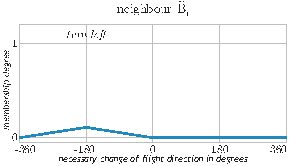
\includegraphics{fig_attractionFLScombined_a}\hspace*{2mm}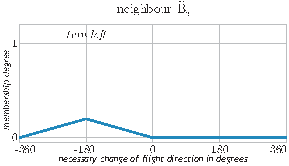
\includegraphics{fig_attractionFLScombined_b}
	\par\vspace*{2mm}
	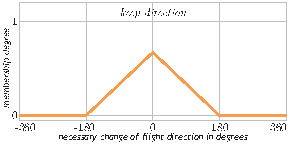
\includegraphics{fig_attractionFLScombined_c}\hspace*{2mm}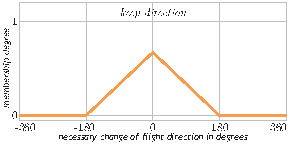
\includegraphics{fig_attractionFLScombined_d}
	\par\vspace*{2mm}
	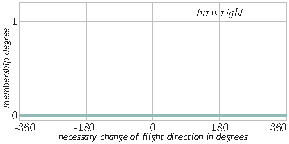
\includegraphics{fig_attractionFLScombined_e}\hspace*{2mm}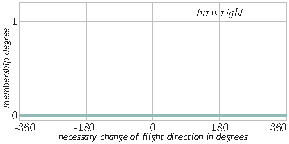
\includegraphics{fig_attractionFLScombined_f}
	\par\vspace*{2mm}
	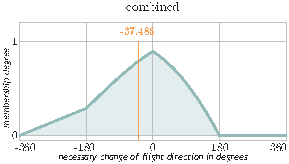
\includegraphics{fig_attractionFLScombined_g}
	\par\vspace*{2mm}
	\caption{The modified output fuzzy sets that result from active rules and represent the flight direction change candidates. They were obtained by evaluating the attraction drive fuzzy rule base for the case when the only two perceived neighbours are 80\% of the visual range away with an angular offset of \ang{-30} ($\fautom{B}_1$), and 60\% of the visual range away with an angular offset of \ang{-110} ($\fautom{B}_2$). The combined fuzzy set is the algebraic sum fuzzy union of the modified output fuzzy sets. The defuzzified value, obtained by using the centroid method, equals \ang{-37.485}.}
	\label{fig:attraction:FLS:combined}
\end{figure}

Even though the combined fuzzy set represents the flight direction change that will help satisfy the attraction drive it is still a fuzzy set. Therefore, in the final step, it has to be converted into a single (crisp) value that is, in some sense, the best representative of the fuzzy set. This is achieved through defuzzification. In this dissertation the centroid defuzzification method is used, which  returns the single (crisp) value, for which the area under the graph of the membership function of the combined fuzzy set is divided into two equal subareas (see subsection~\ref{subsec:fuzzyModelling:fuzzyRuleBase}).

If I return to the example: the defuzzified value resulting from the combined fuzzy set presented in figure~\ref{fig:attraction:FLS:combined} is \ang{-37.485}. This means that in order to satisfy the fuzzy attraction drive, the fuzzy animat should turn to the left by \ang{37.485}. By computing the necessary change in flight speed it can be found out that the fuzzy animat, in order to satisfy the fuzzy attraction drive, should also increase its flight speed by 17.3489\% of its maximal achievable flight speed.\footnote{It is important to note that if the fuzzy animat is already flying at its maximal achievable flight speed, it will keep on flying at this speed and the desired increase will remain unaccomplished. This will happen due to the truncation of the flight speed in the fuzzy weighted sum action selection function.} The fuzzy repulsion drive would be satisfied with a turn to the right by \ang{11.078} and a speed increase of 4.3825\% of its maximal achievable flight speed. Since the fuzzy animat and the perceived neighbours have the same flight direction and flight speed, the fuzzy alignment drive does not require any changes (\fig~\ref{fig:attraction:FLS:output}). 

\begin{figure}
	\null\vspace*{.5\gridH}
	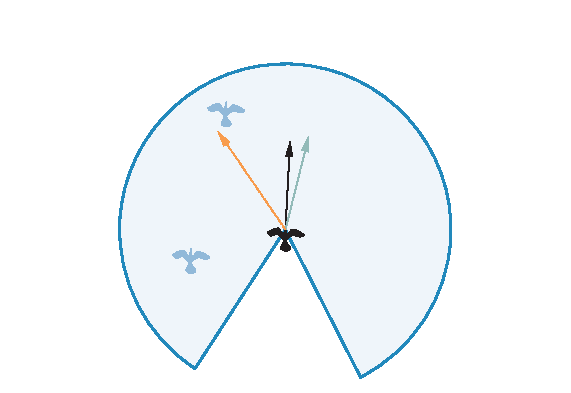
\includegraphics{fig_attractionFLSout}
	\vspace*{.5\gridH}
	\caption{The defuzzified desired flight direction and flight speed changes in the case when the observed fuzzy animat perceives only two neighbours. One neighbour is 80\% of the visual range away with an angular offset of \ang{-30}, and the other 60\% of the visual range away with an angular offset of \ang{-110}. All have the same flight direction and flight speed. The orange arrow represents the flight direction and flight speed change that would satisfy the fuzzy attraction drive, while the green arrow represents the flight direction and speed change that would satisfy the fuzzy repulsion drive.}
	\label{fig:attraction:FLS:output}
\end{figure}
